\samerowans{\begin{problem}{1}
$KE$ --- биссектриса $\angle{CKB}$, $\angle{CKE} = 40^{\text{o}}$, $DK \perp CK$. Найдите $\angle{AKD}$.
\end{problem}} 

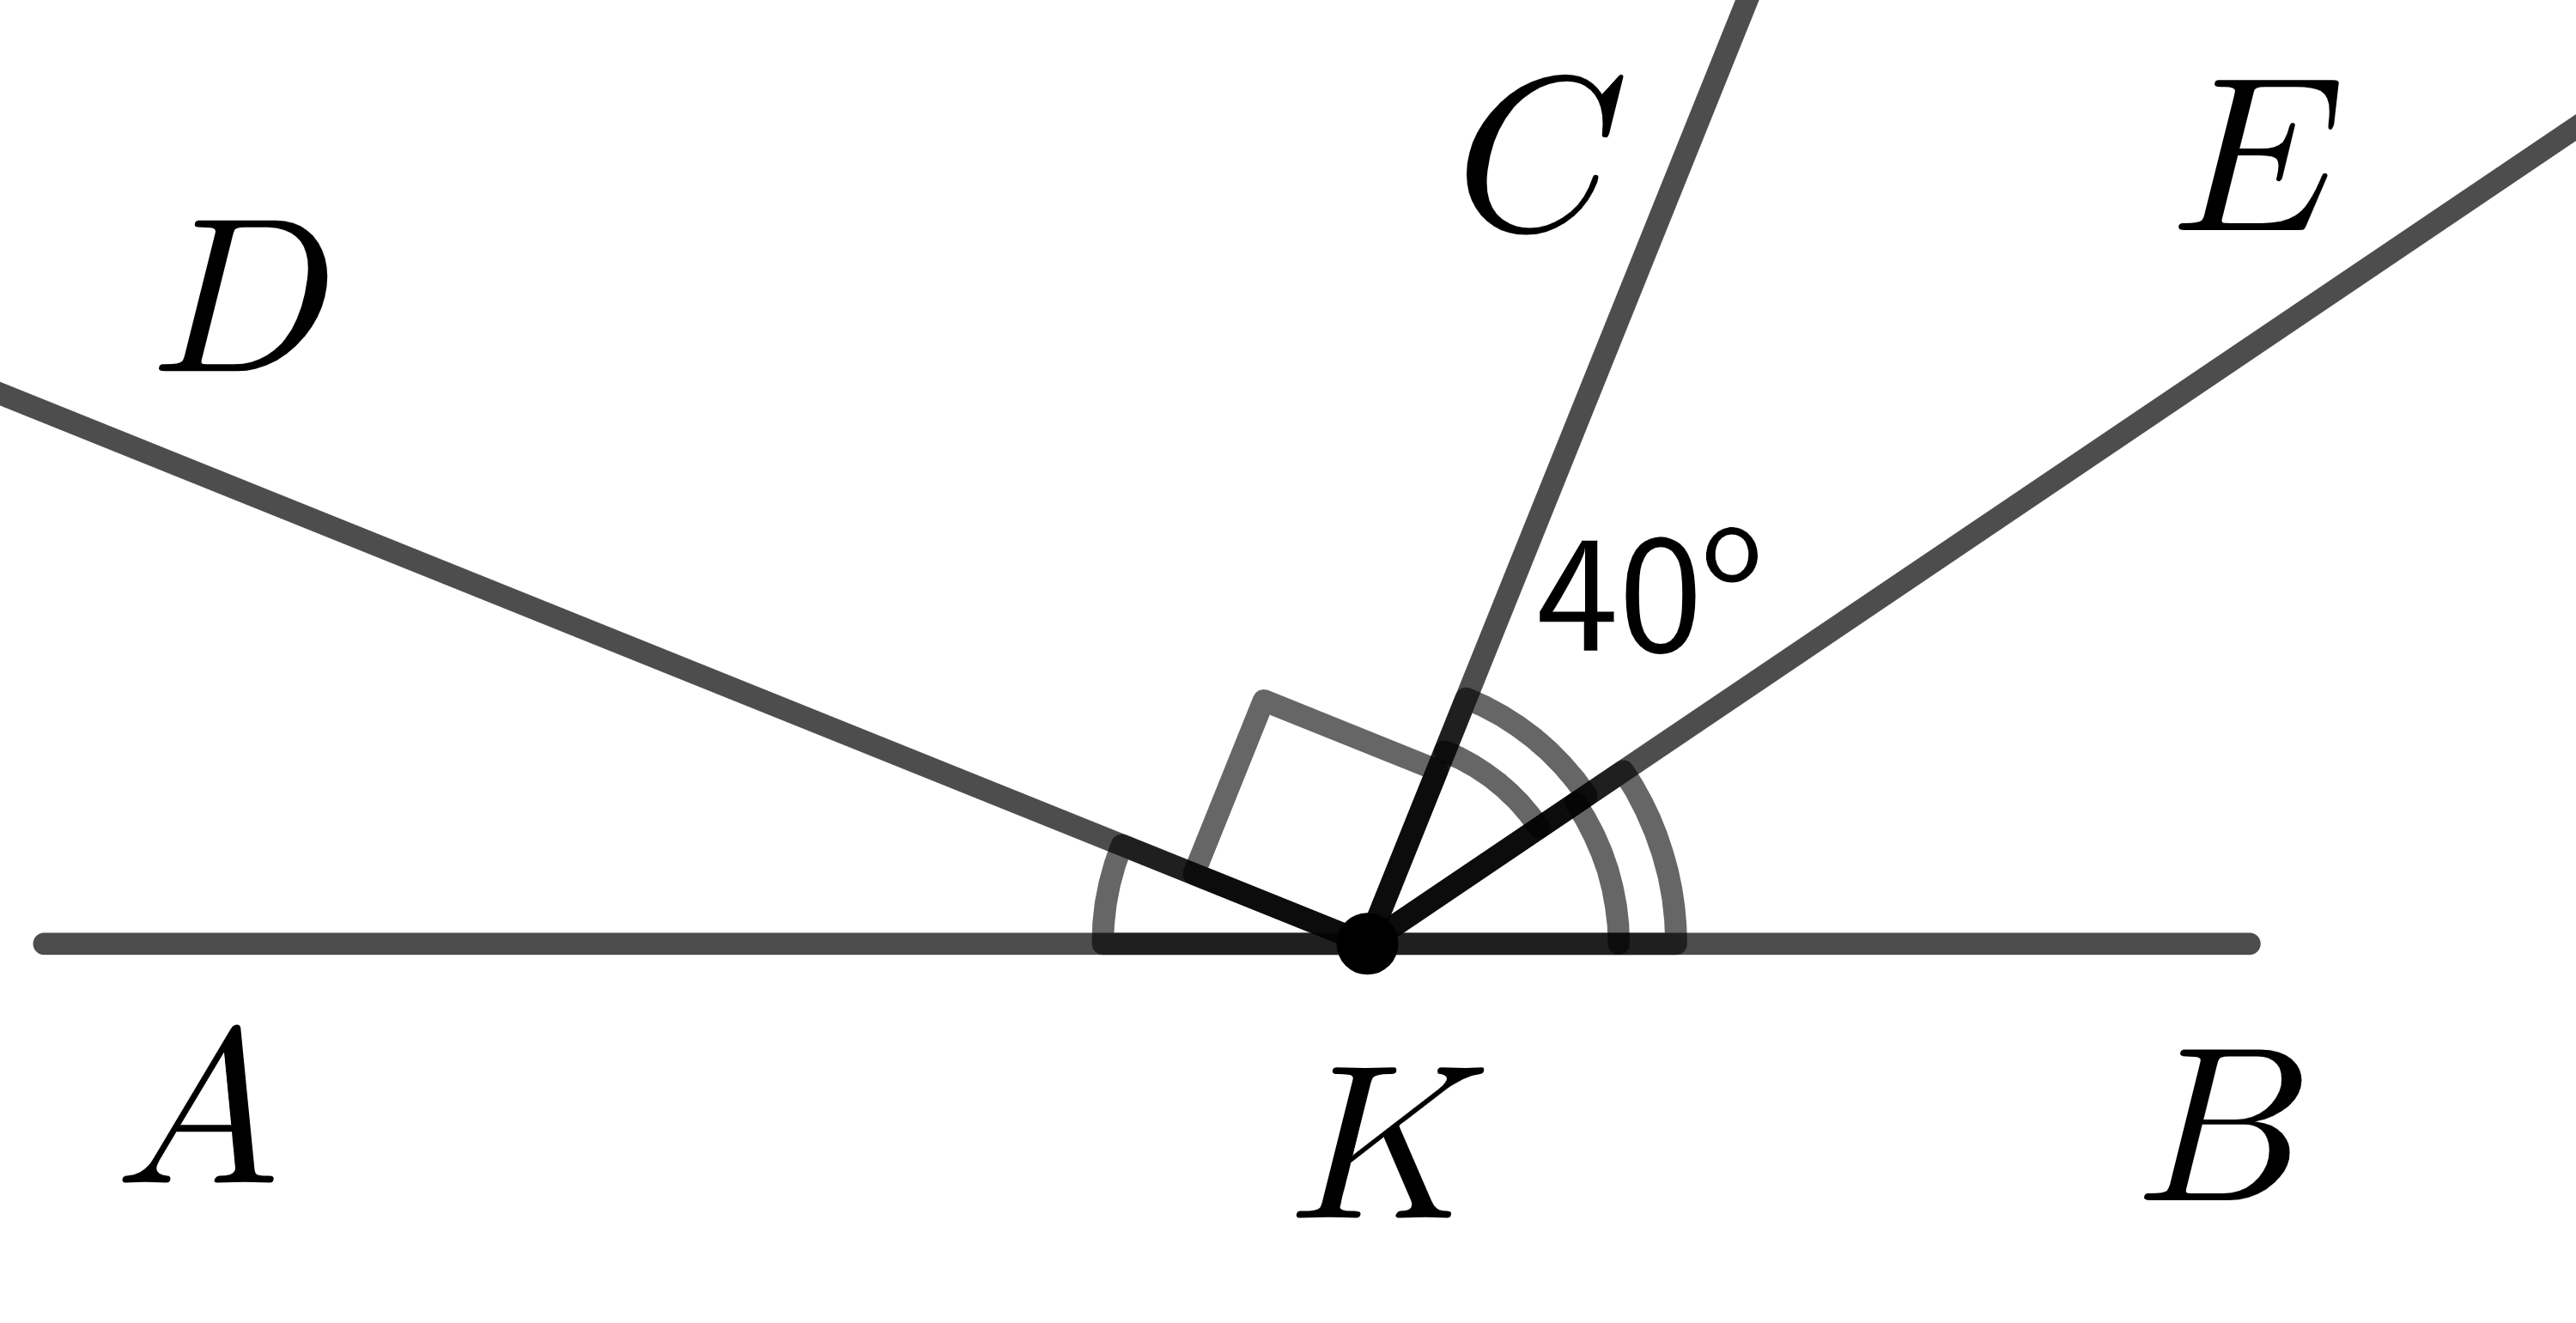
\includegraphics[width=.3\textwidth]{20260404/pics/20260404_geom_for_mat_01_v1.png}

\samerowans{\begin{problem}{2a}
Прямые $a$ и $b$ параллельны. По данным чертежа найдите неизвестные углы $x$, $y$ и $z$.
\end{problem}} 

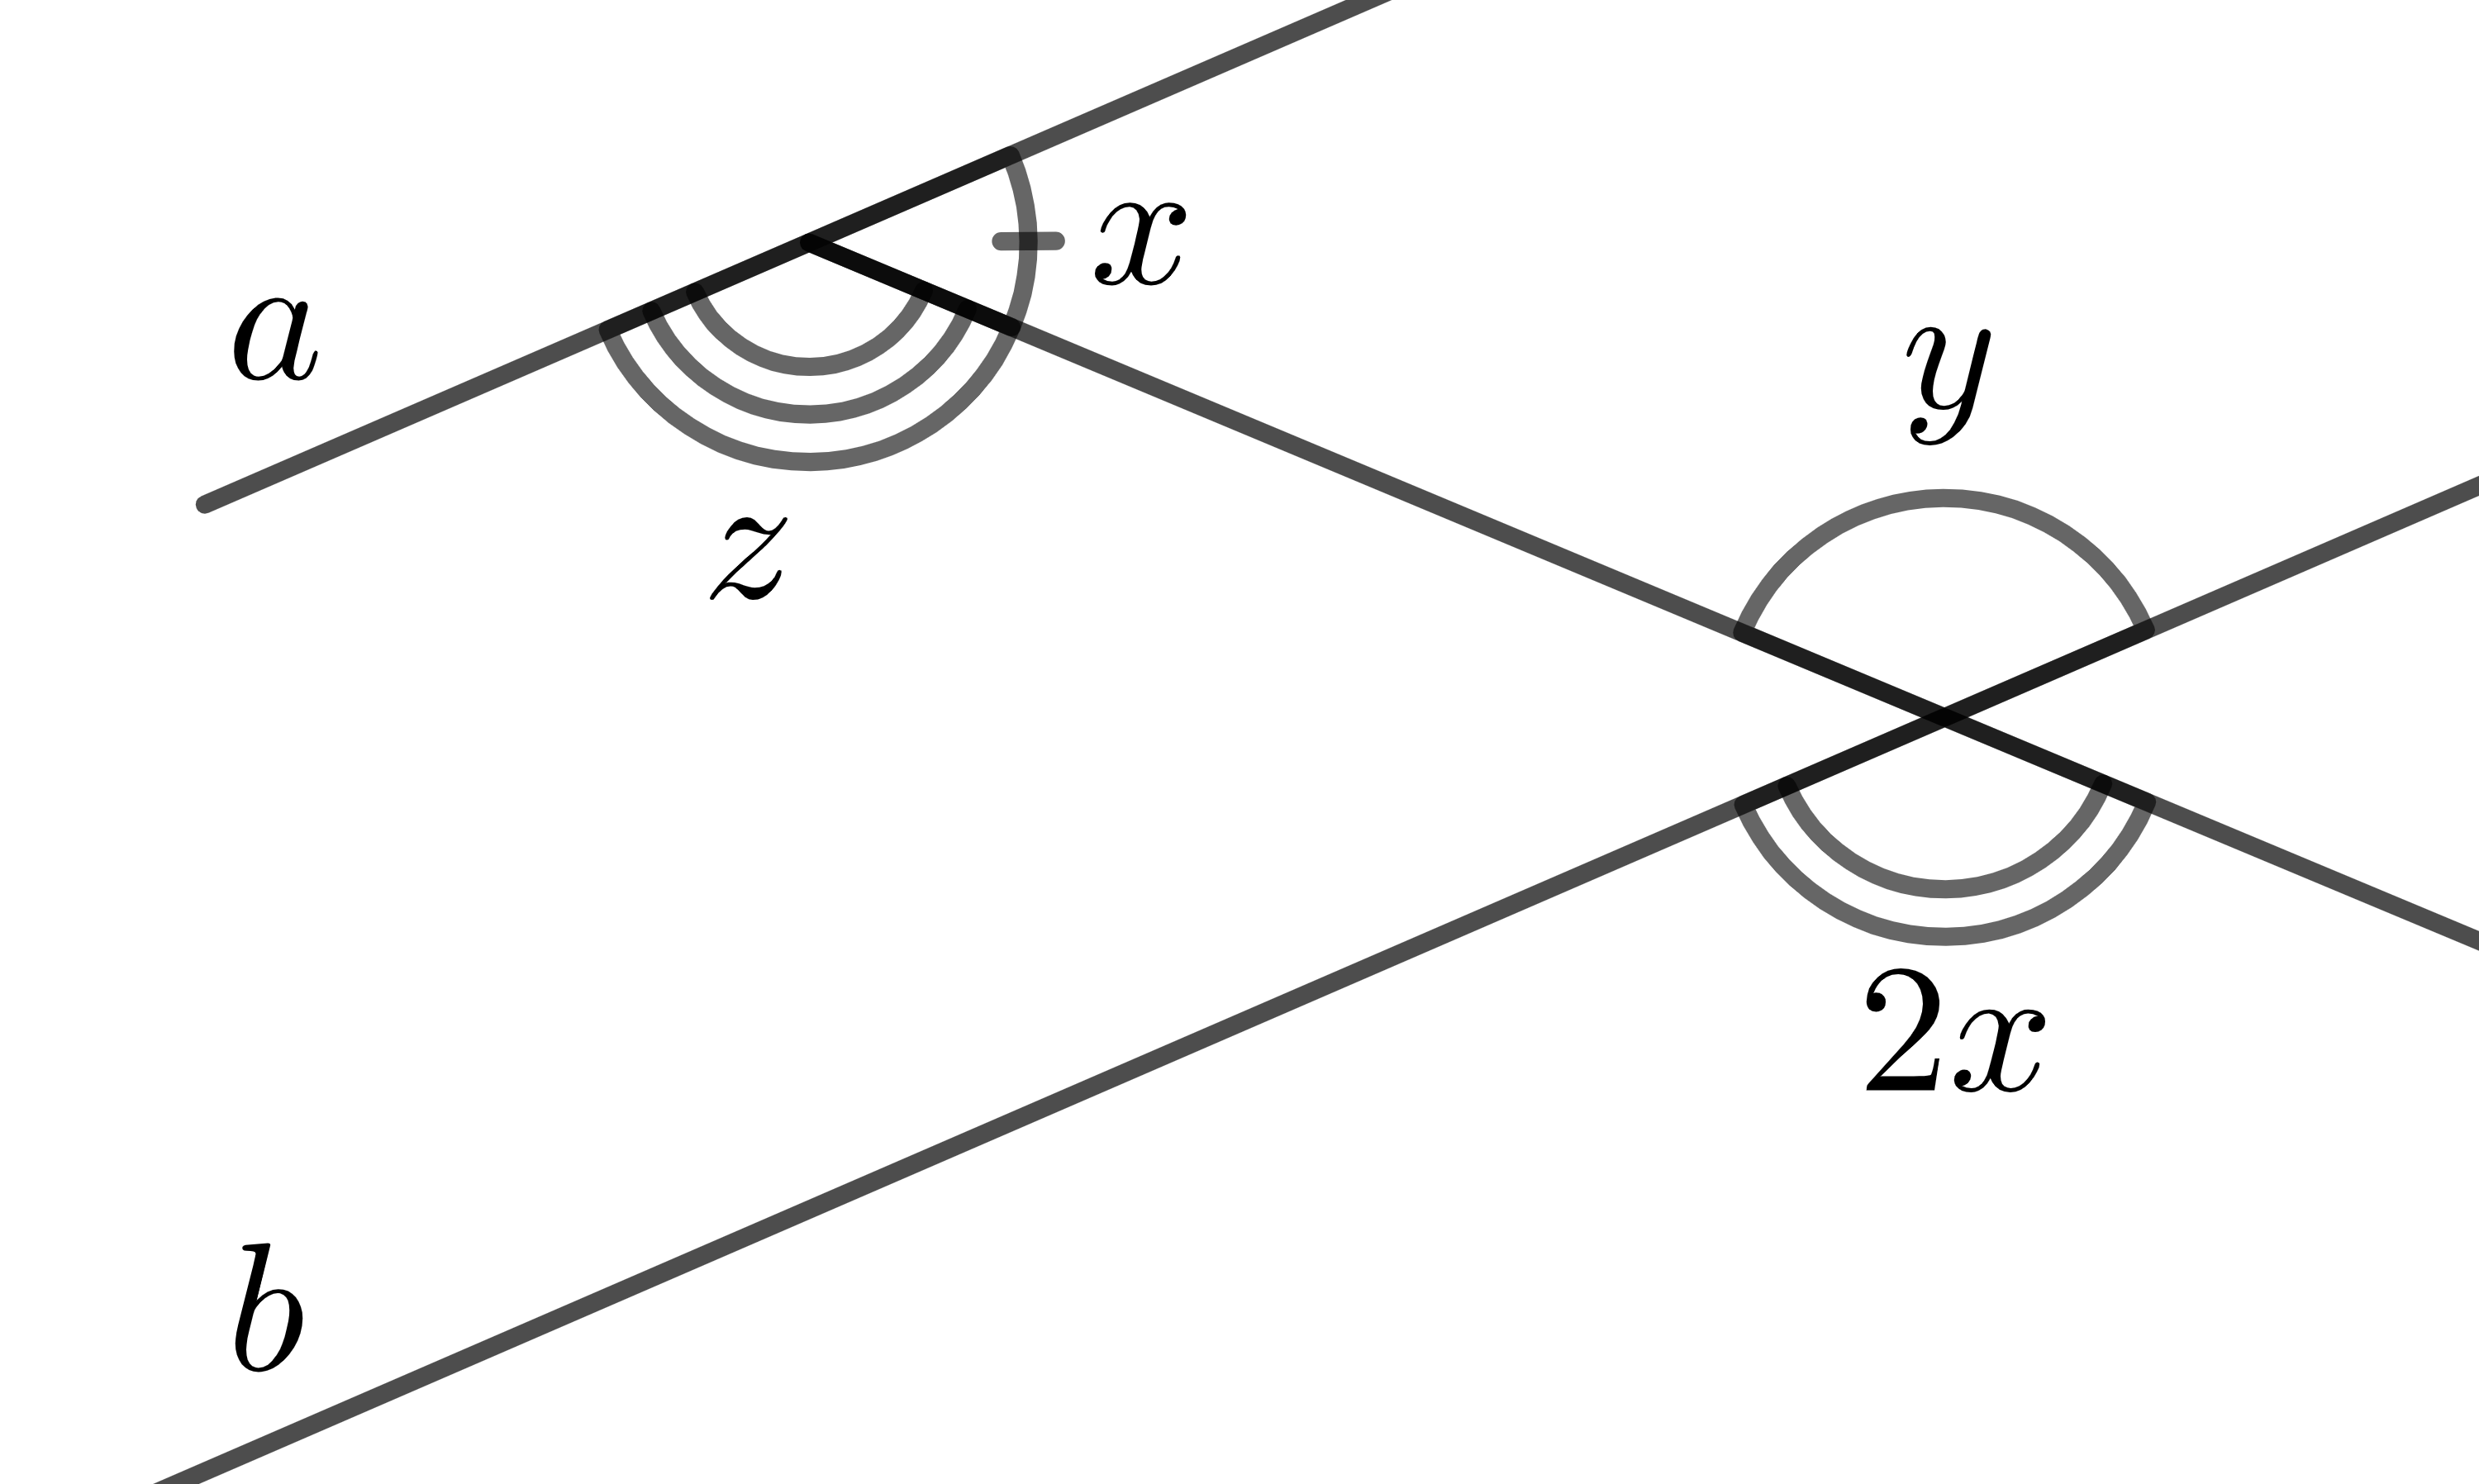
\includegraphics[width=.3\textwidth]{20260404/pics/20260404_geom_for_mat_02a_v1.png}

\samerowans{\begin{problem}{2b}
Прямые $a$ и $b$ параллельны. По данным чертежа найдите неизвестные углы $x$, $y$ и $z$.
\end{problem}} 

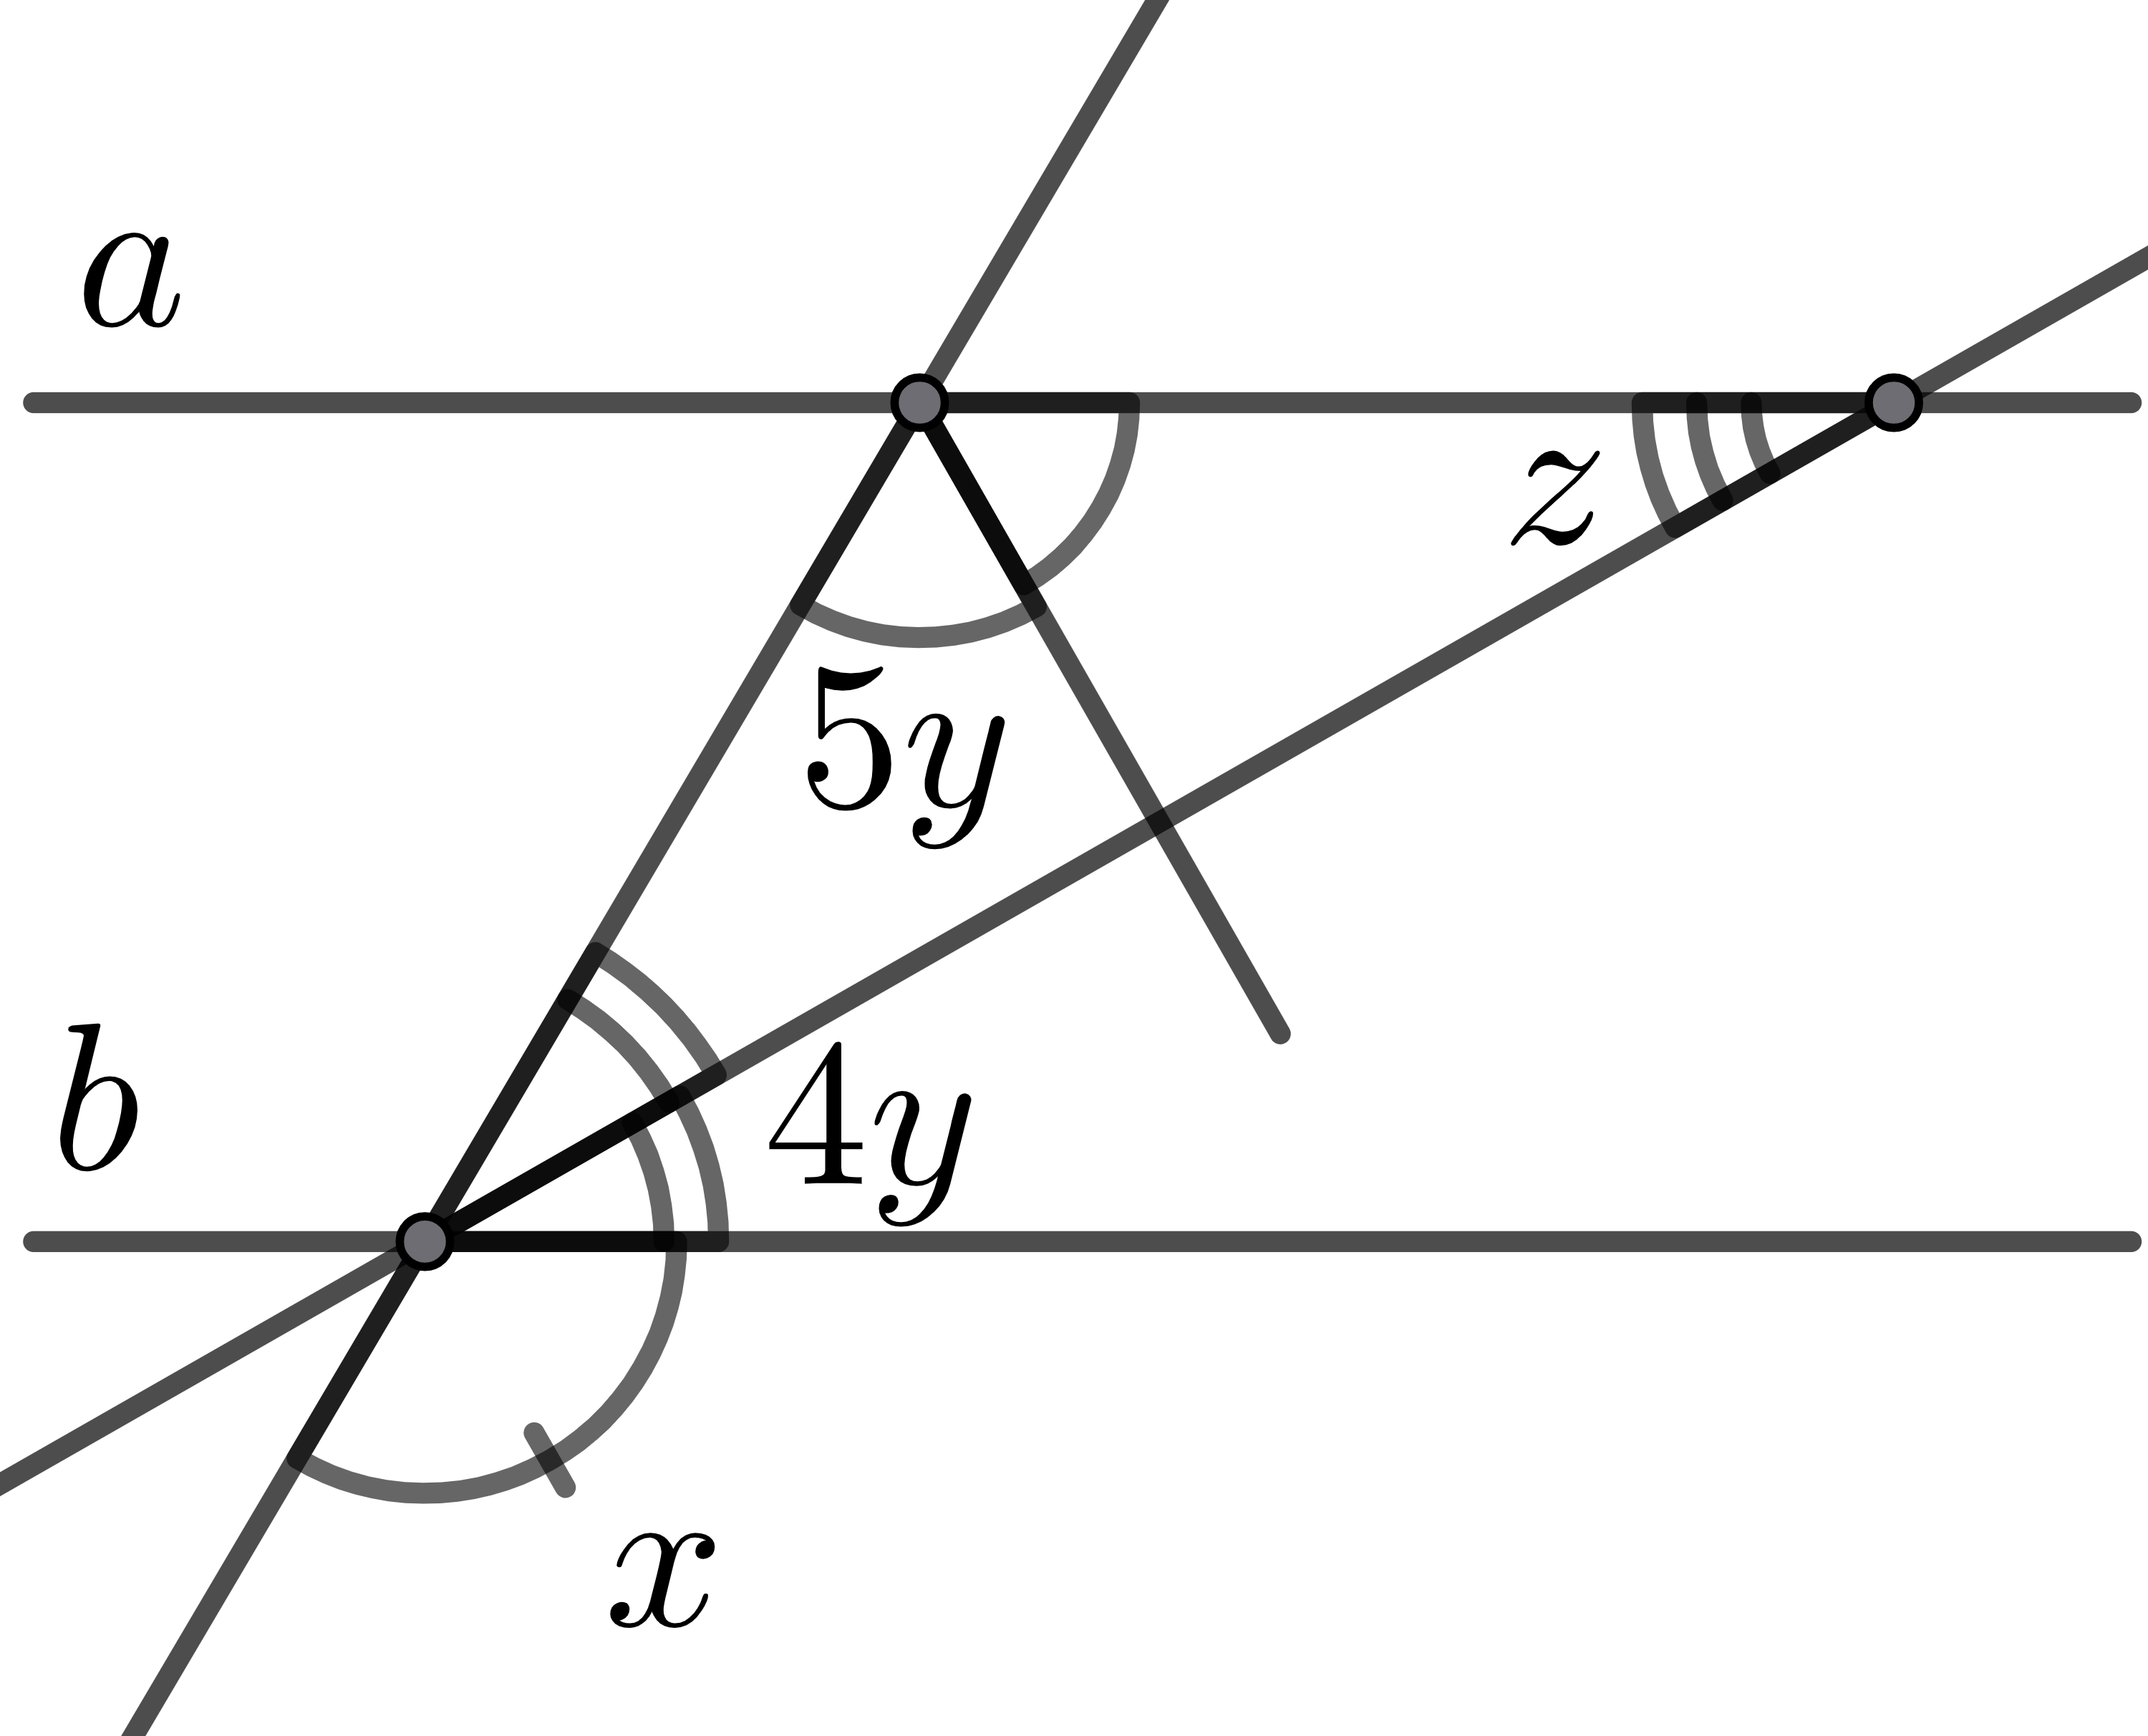
\includegraphics[width=.3\textwidth]{20260404/pics/20260404_geom_for_mat_02b_v1.png}

\samerowans{\begin{problem}{3}
Через точку пересечения биссектрис $\triangle{ABC}$ проведена прямая, параллельная прямой $AC$, пересекающая стороны $AB$ и $BC$ в точках $M$ и $N$ соответственно. $MN=12$, $AM$ на 6 меньше $NC$. Найдите длину $NC$.
\end{problem}} 

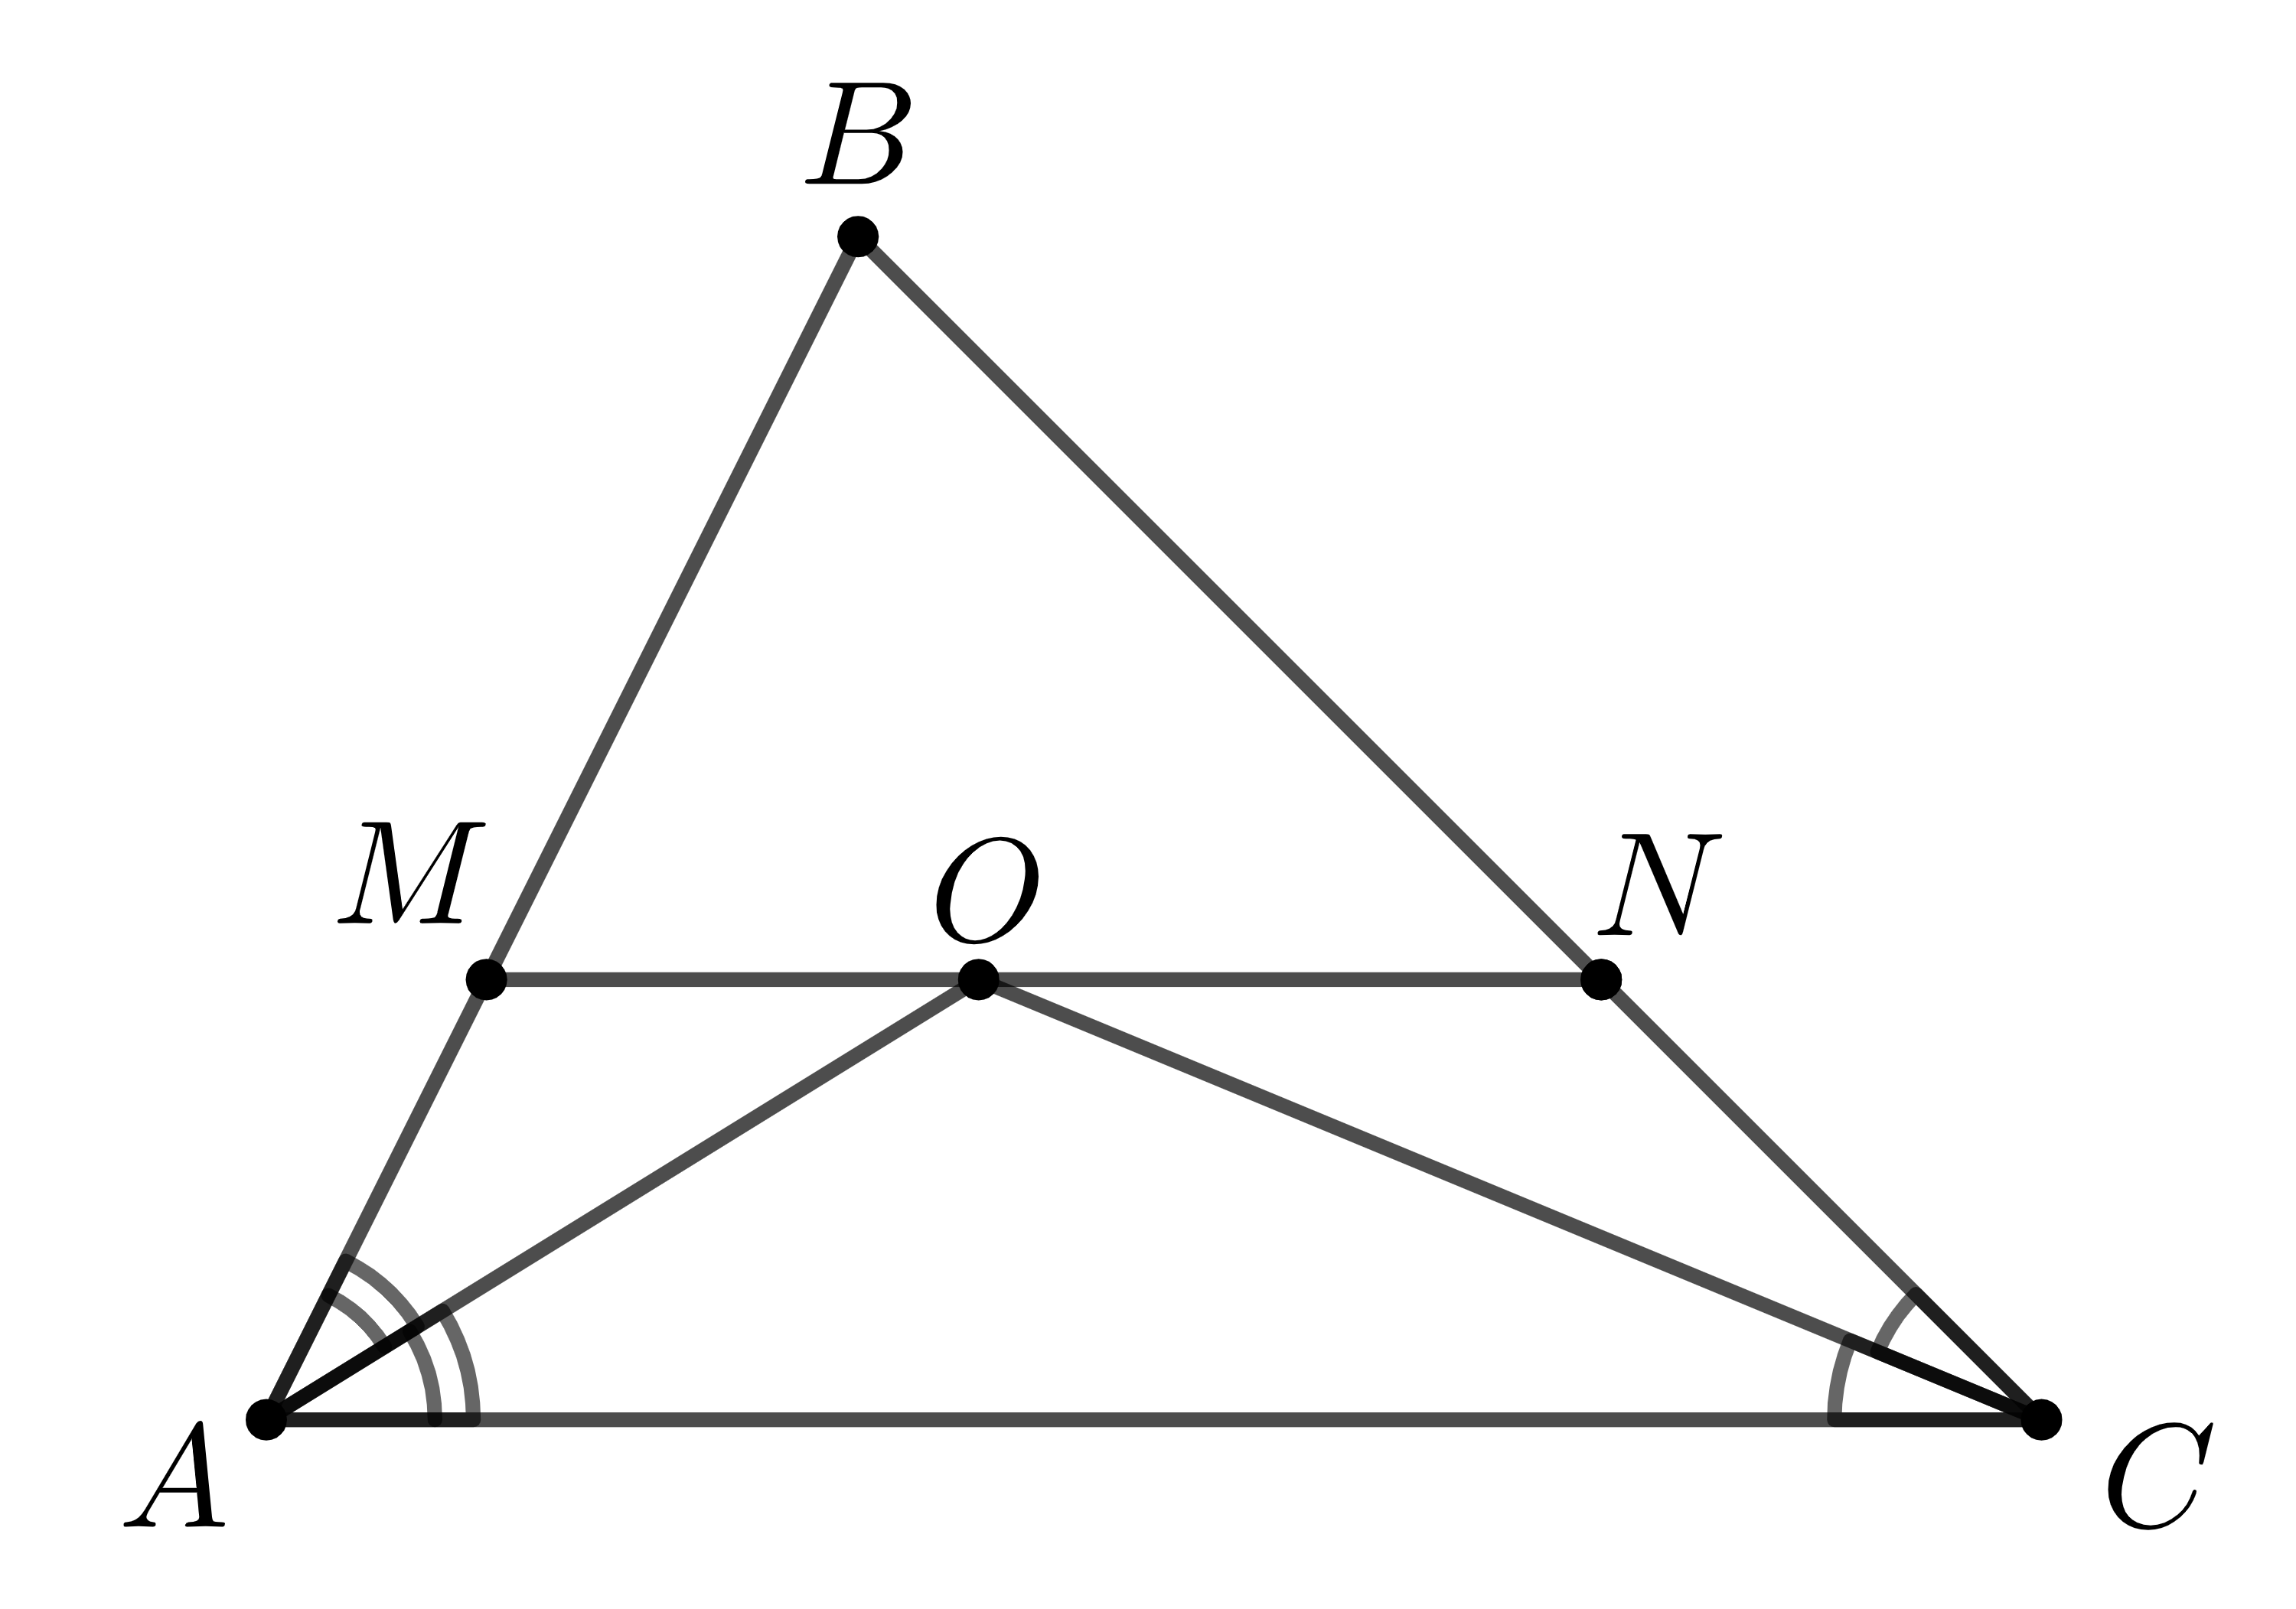
\includegraphics[width=.3\textwidth]{20260404/pics/20260404_geom_for_mat_03_v1.png}

\samerowans{\begin{problem}{4}
Дан равносторонний $\triangle{ABC}$. На стороне $AC$ взята точка $M$ такая, что сумма периметров треугольников $ABM$ и $MBC$ равна 48 см. Найдите длину стороны $\triangle{ABC}$,  если $MB=9\text{ см}$.
\end{problem}} 

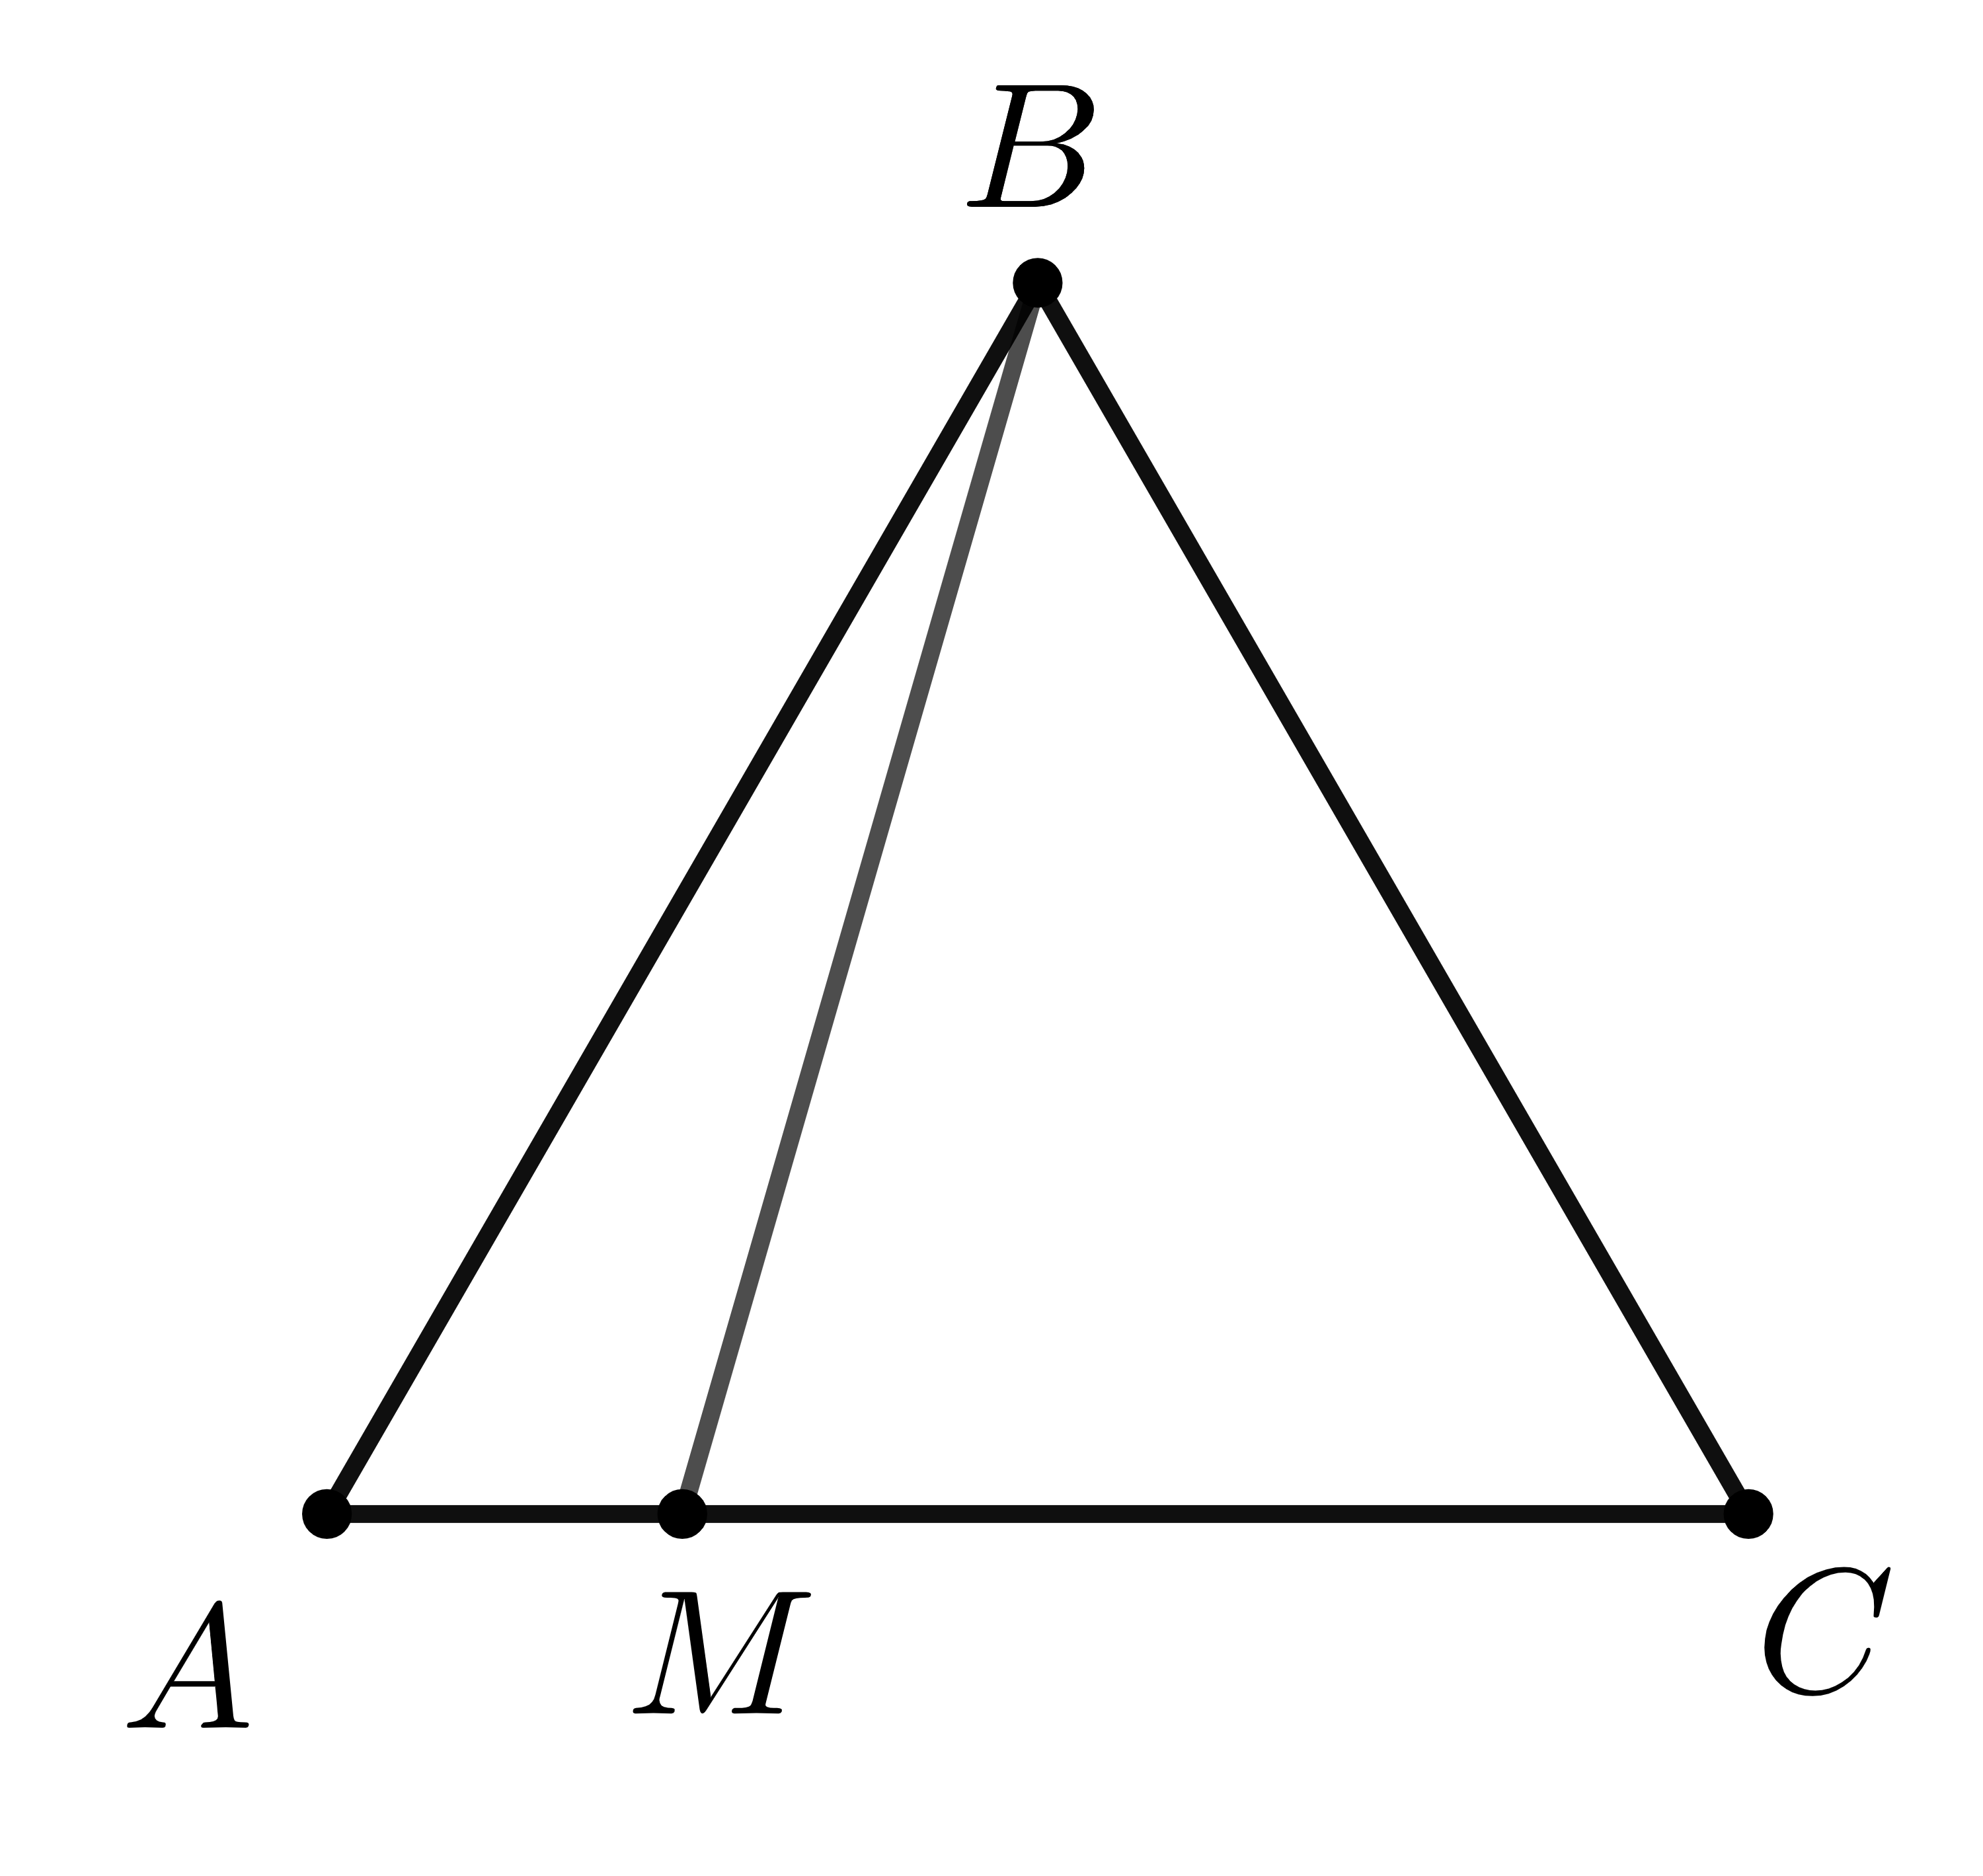
\includegraphics[width=.3\textwidth]{20260404/pics/20260404_geom_for_mat_04_v1.png}

\samerowans{\begin{problem}{5}
Точка $P_1$ --- середина отрезка $CD$. Точка $P_2$ --- середина отрезка $P_1D$. Точка $P_3$ --- середина отрезка $P_2D$. Точка $P_4$ --- середина отрезка $P_3D$. Длина отрезка $P_1P_4=21$ см. Найдите длину отрезка $CD$. 
\end{problem}} 

\samerowans{\begin{problem}{6}
Выпишите номера верных утверждений. Если верных нет --- напишите 0.
\end{problem}} 

1) Если разность двух сторон и периметр одного треугольника равны разности двух сторон и периметру другого треугольника, то эти треугольники равны. 

2) Если стороны углов соответственно параллельны, то углы равны.

3) Медиана треугольника может равняться соседней стороне.

4) Существует прямая, которая перпендикулярна каждой из двух пересекающихся прямых.


\samerowans{\begin{problem}{7}
Известно, что $\angle{A} = 35^{\text{o}}$, $\angle{B} = 37^{\text{o}}$, $\angle{C} = 42^{\text{o}}$, $\angle{D} = 45^{\text{o}}$. Найдите $\angle{E}$.
\end{problem}} 

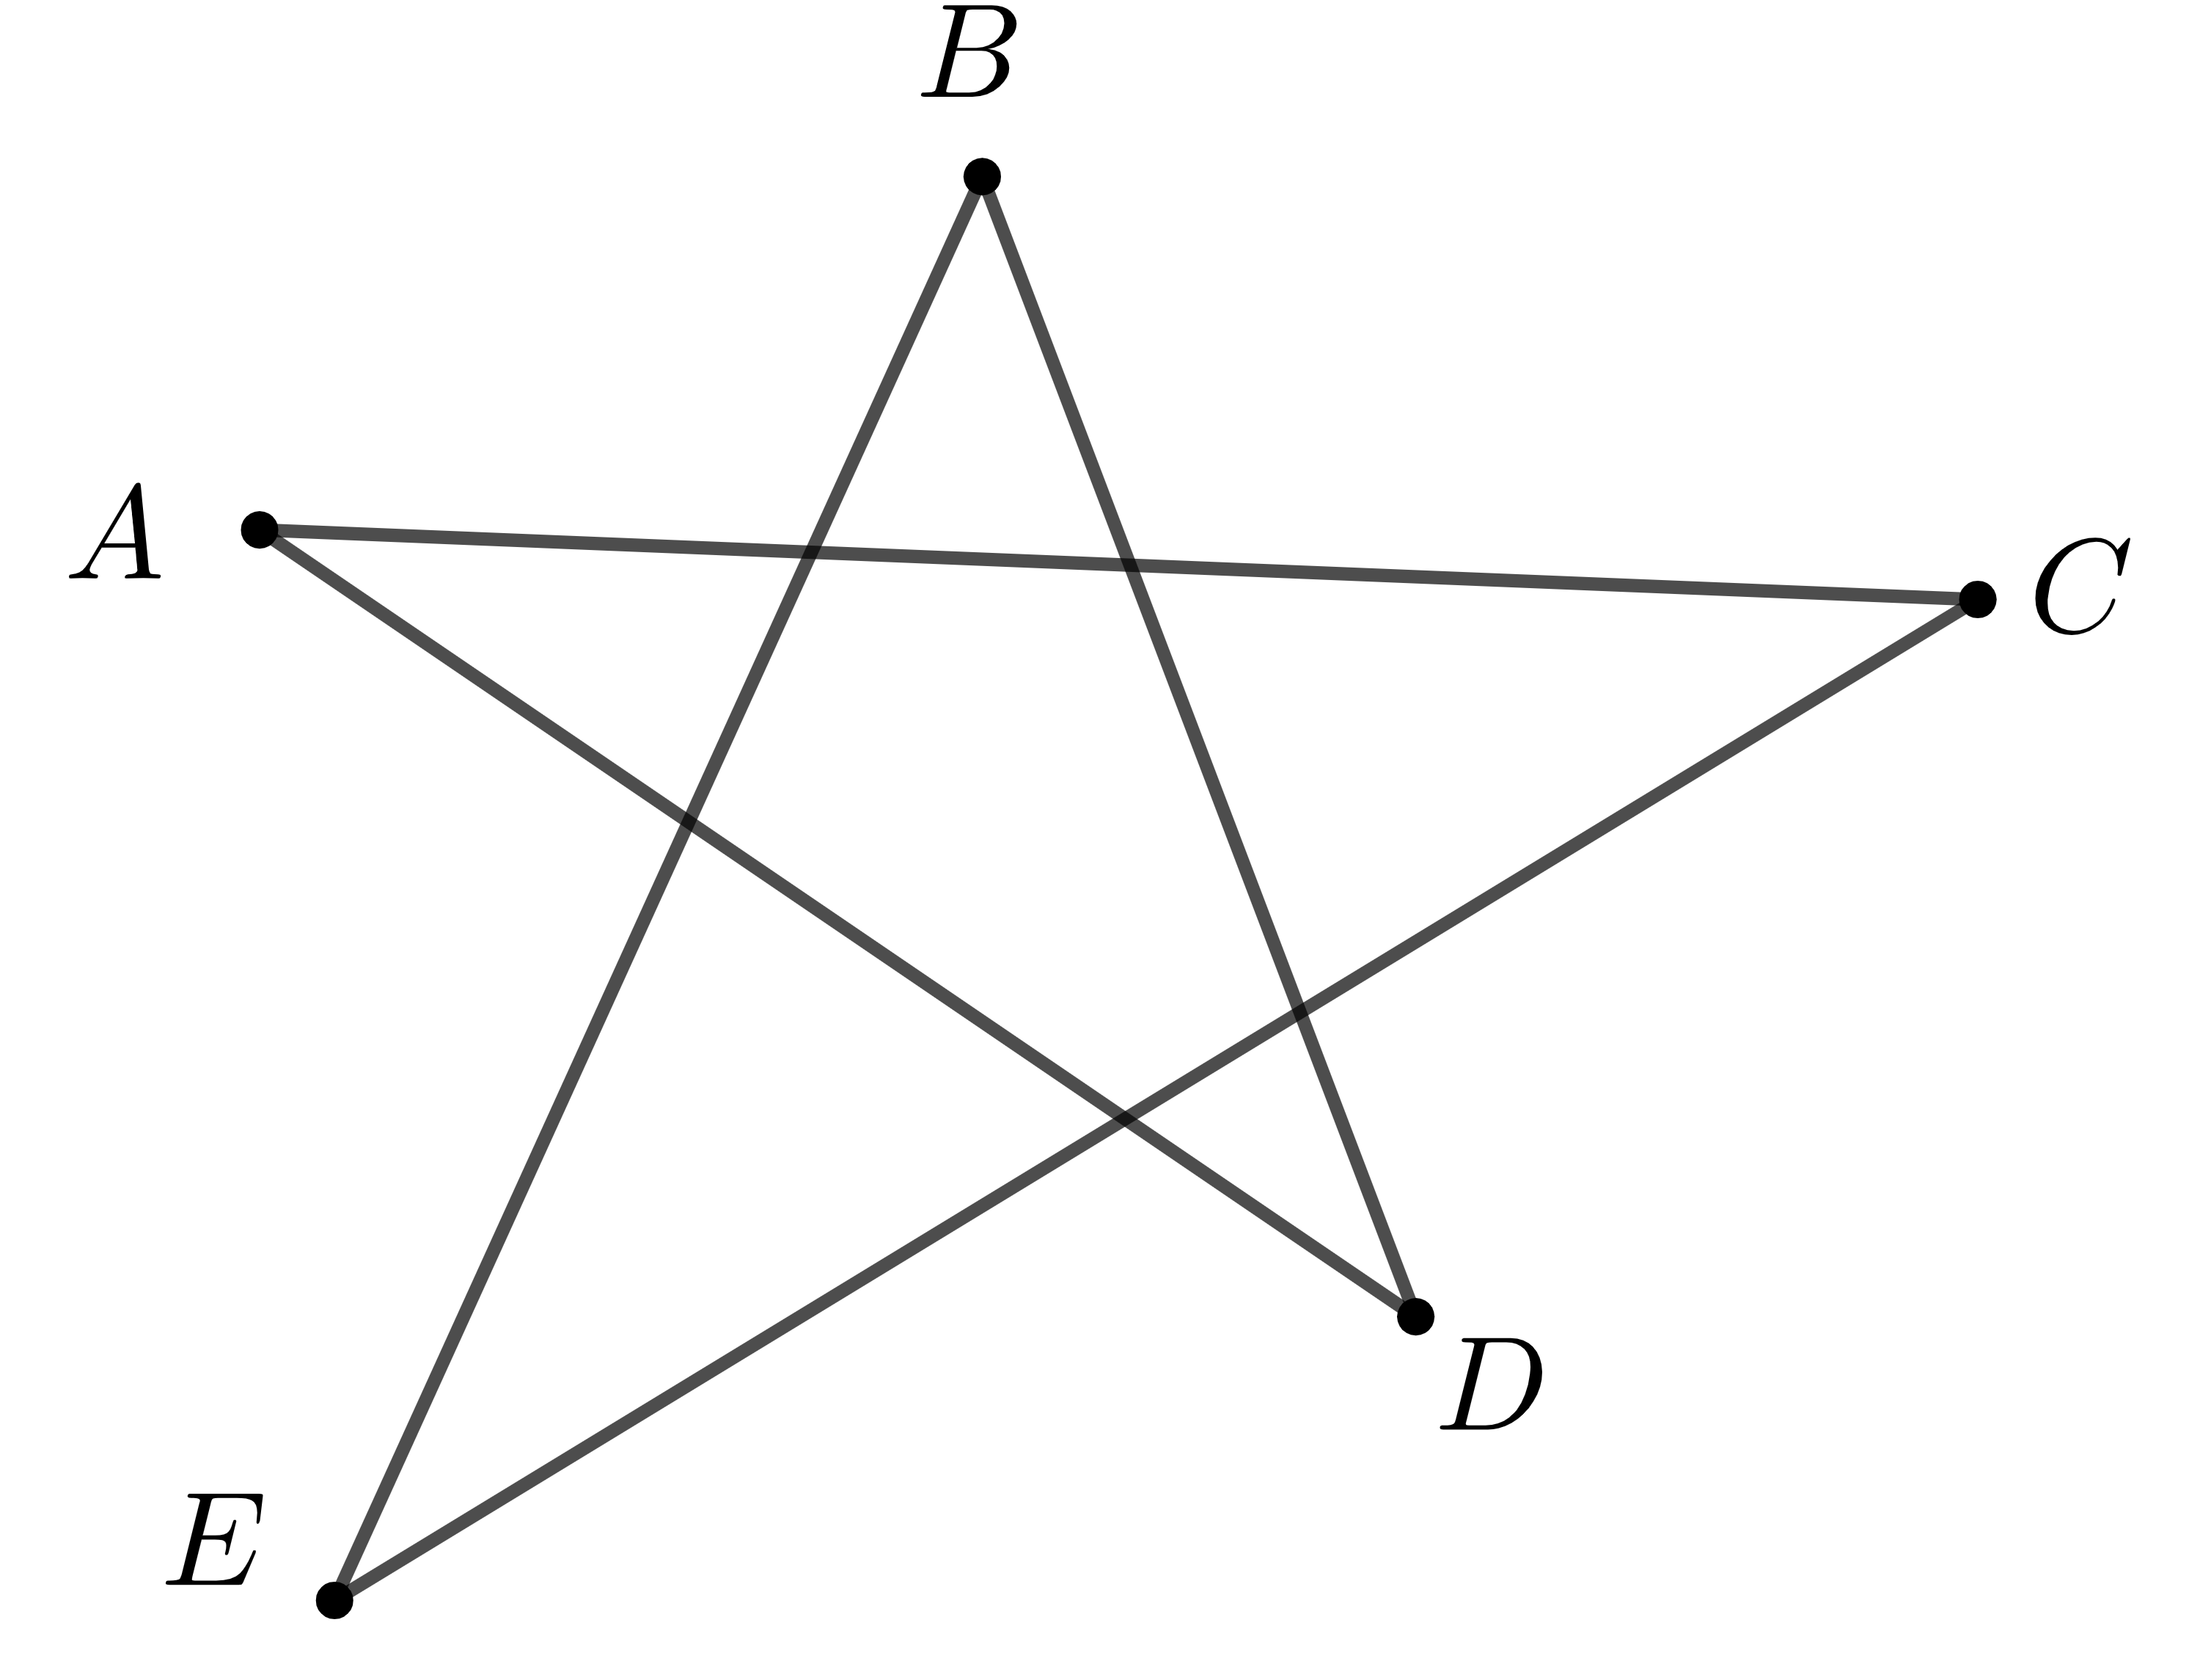
\includegraphics[width=.3\textwidth]{20260404/pics/20260404_geom_for_mat_07.png}

\begin{problem}{8}
На рисунке $\angle{ABC}=90^{\text{o}}$, $\angle{MBA}=45^{\text{o}}$. Докажите, что $\triangle{ABC}$ равнобедренный.
\end{problem}

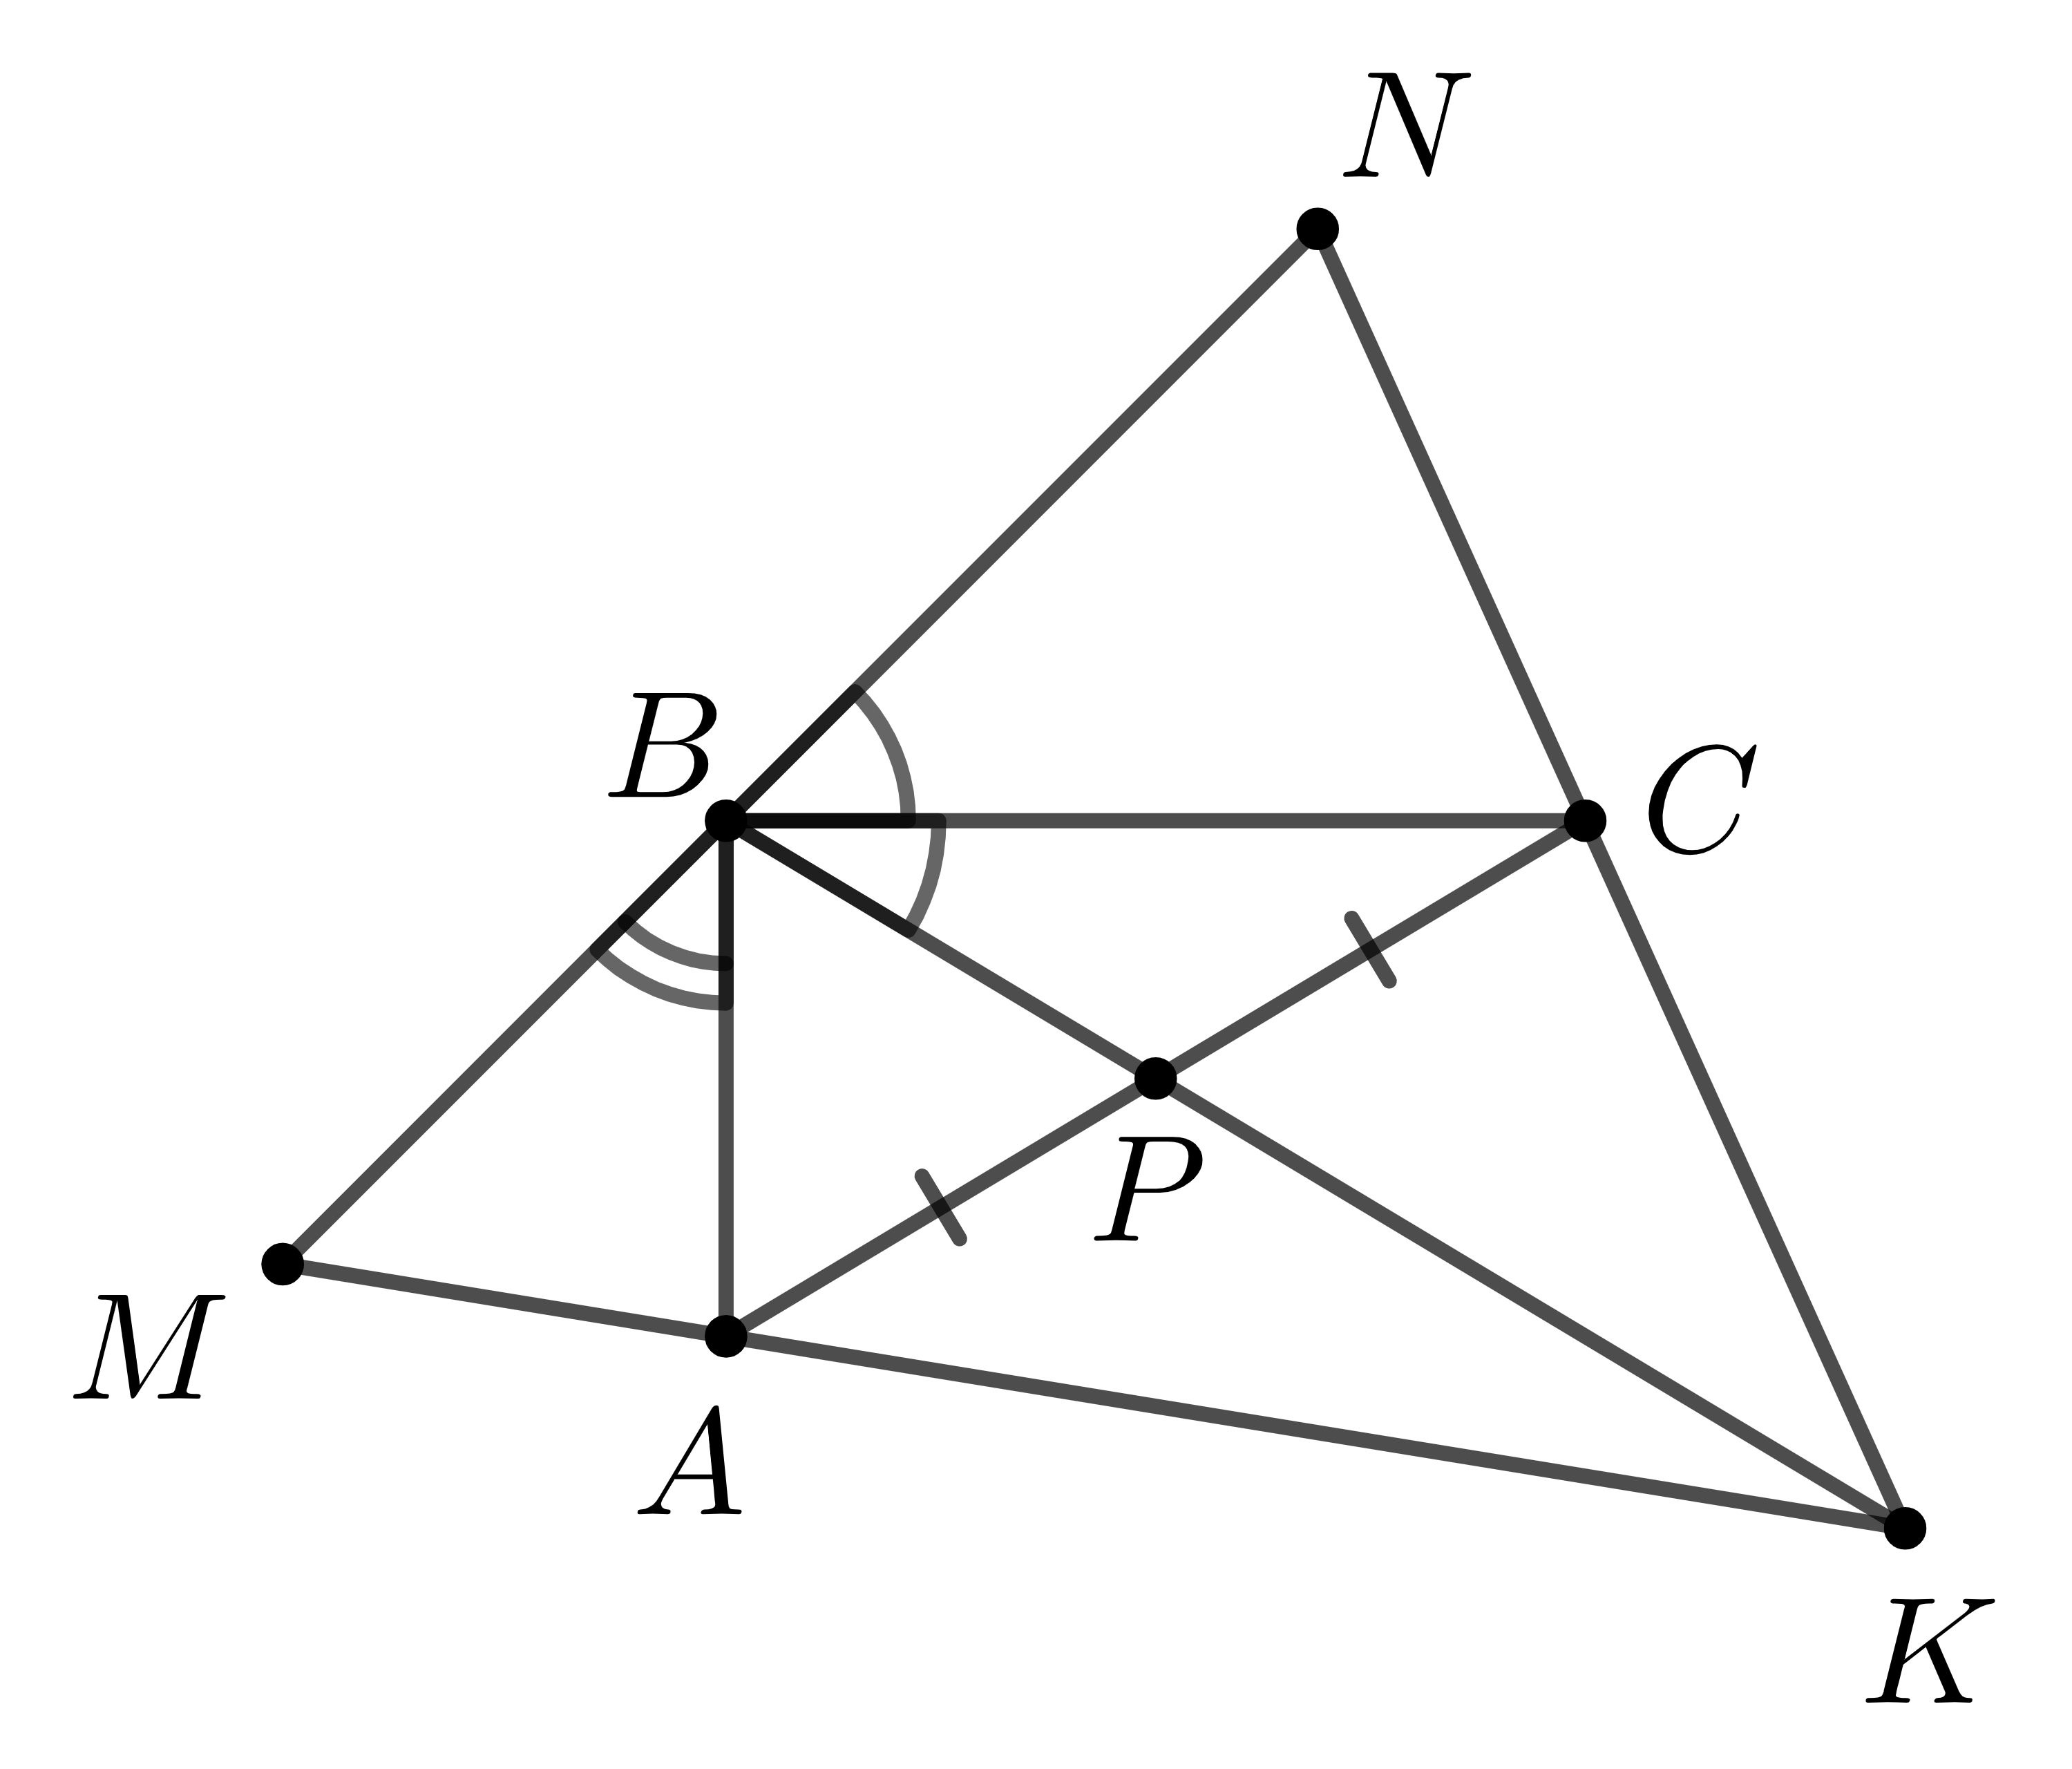
\includegraphics[width=.3\textwidth]{20260404/pics/20260404_geom_for_mat_08.png}

\begin{problem}{9}
Дан четырёхугольник $ABCD$. Известно, что $\angle{CAD}=\angle{DBA}=40^{\text{o}}$, $\angle{CAB=60^{\text{o}}}$, $\angle{CBD}=20^{\text{o}}$. Найдите угол $CDB$.
\end{problem}

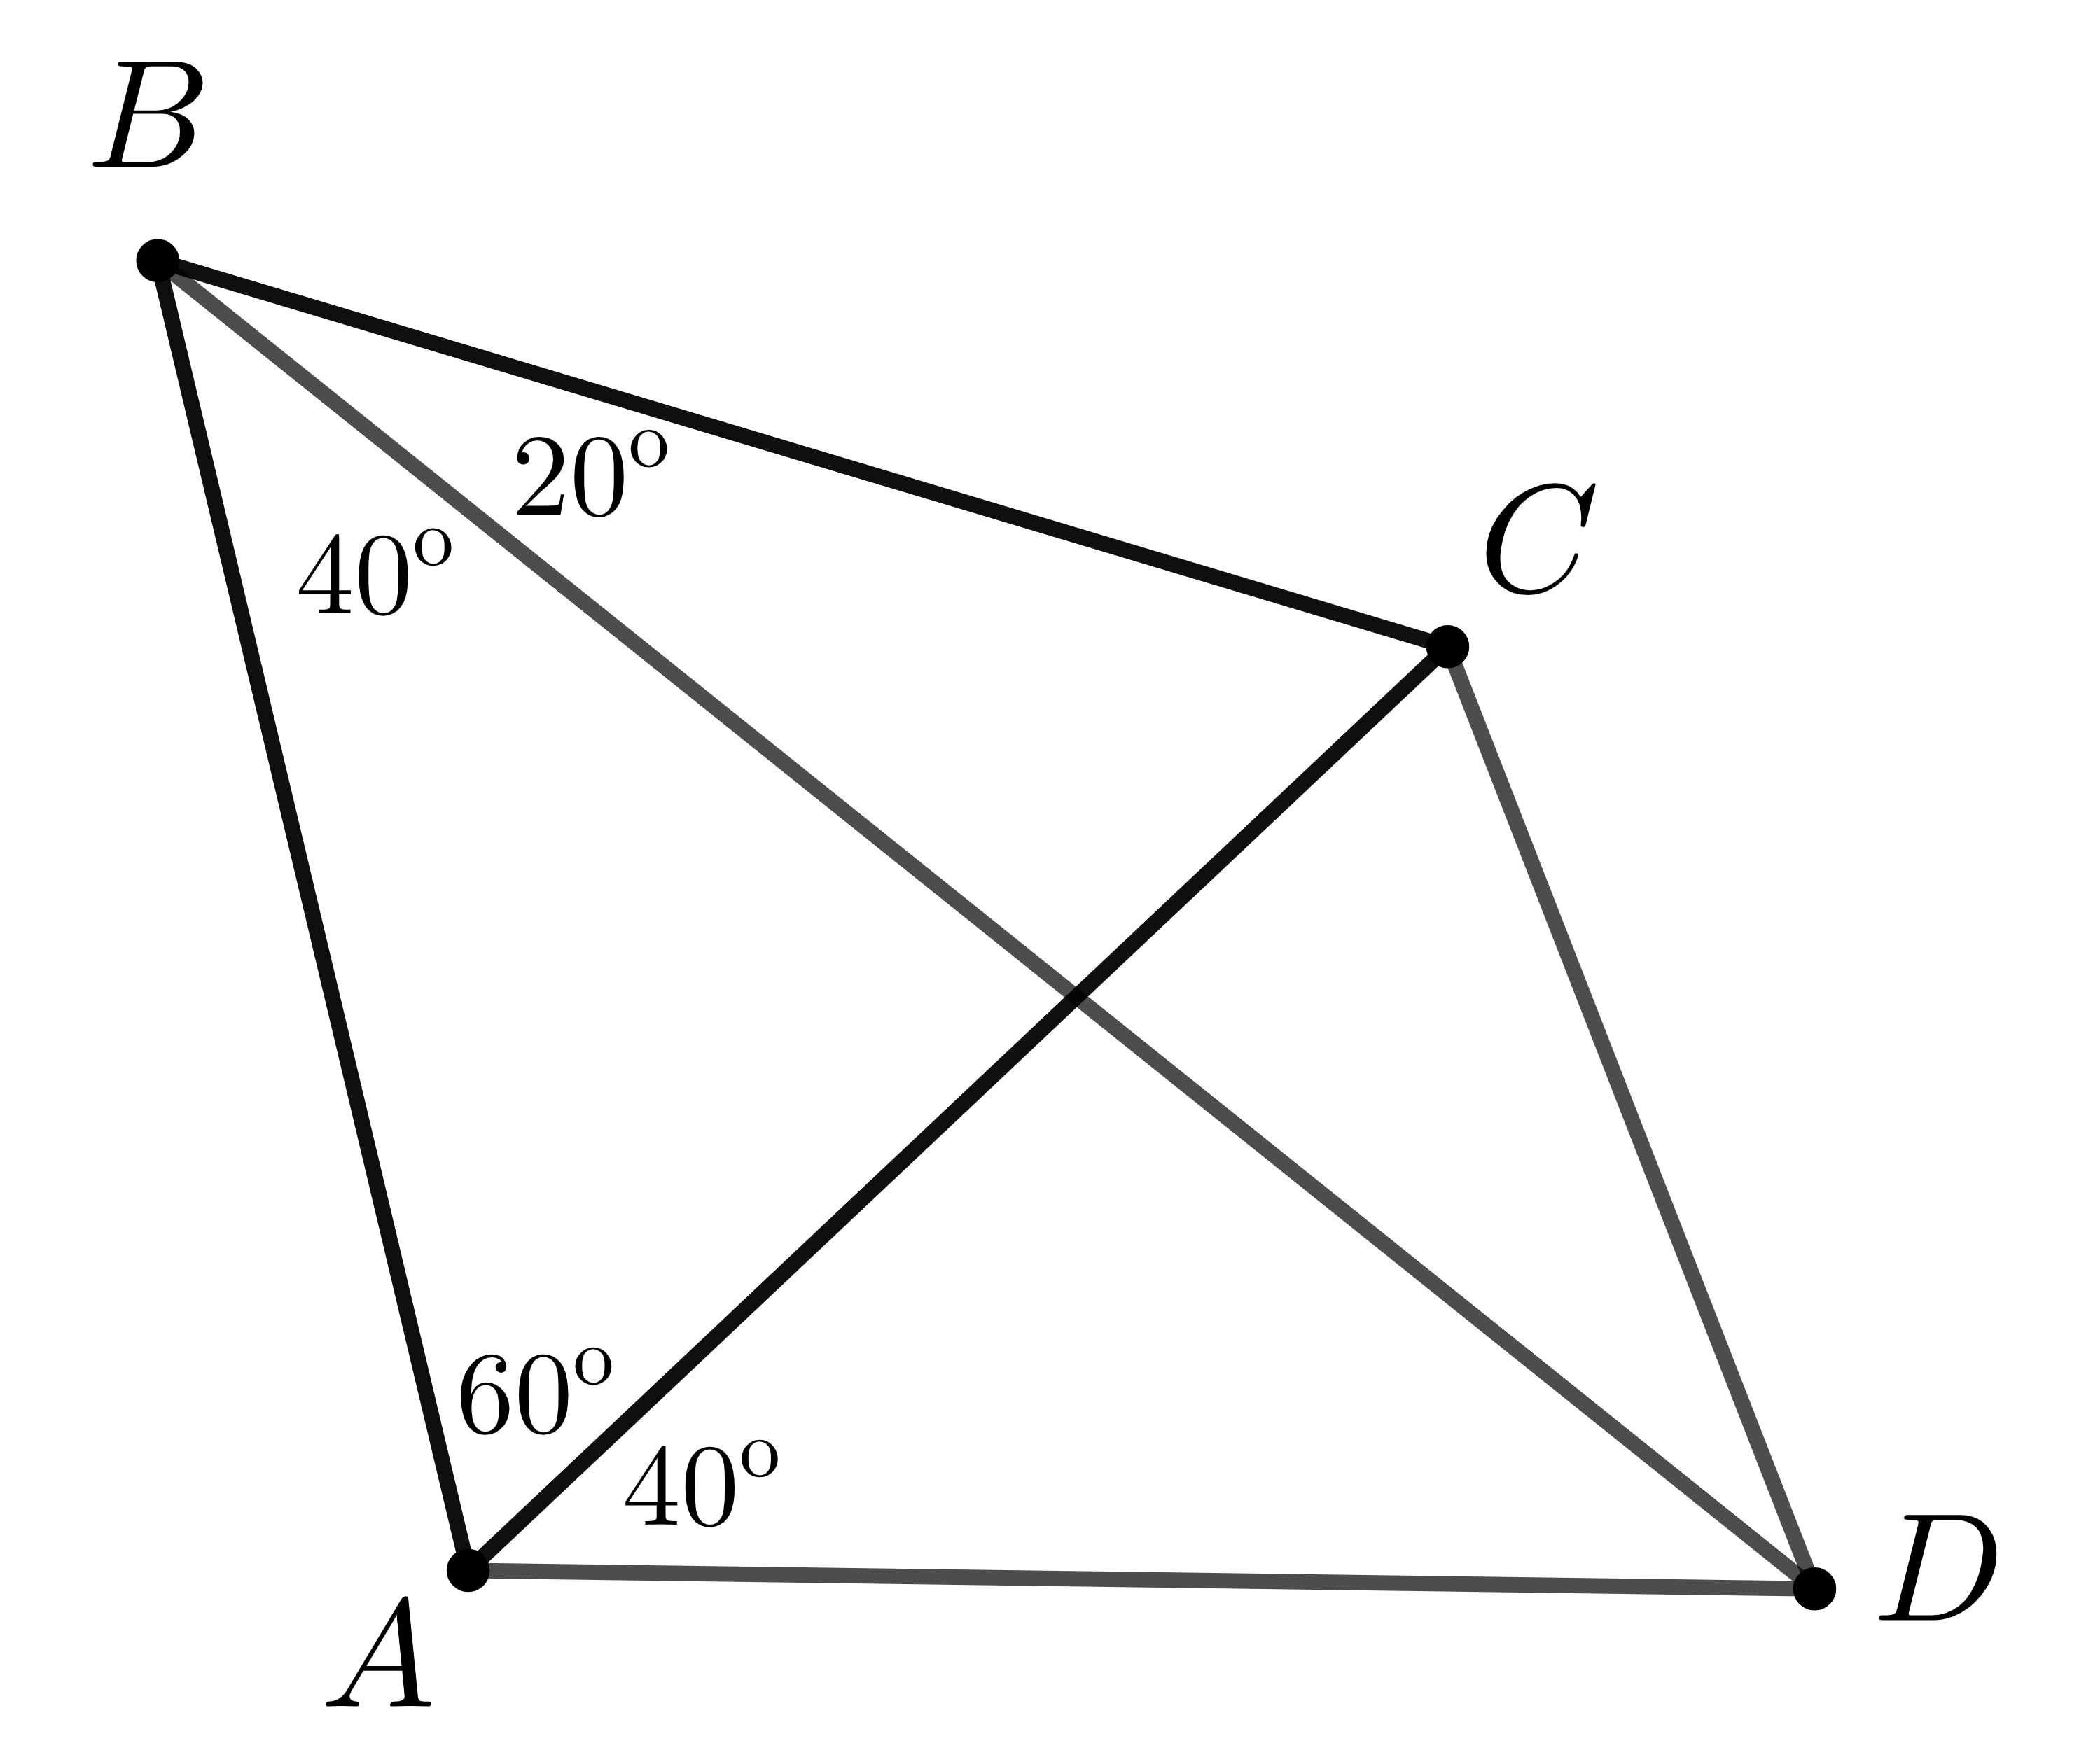
\includegraphics[width=.3\textwidth]{20260404/pics/20260404_geom_for_mat_09_v1.png}

\begin{problem}{10}
На сторонах $BC$ и $CD$ квадрата $ABCD$ взяли точки $K$ и $M$ так, что угол  $MAK$ равен $45^{\text{o}}$. Докажите, что $BK+DM=MK$.  
\end{problem}
